%%%% Paramétrage du TD %%%%
\def\xxactivite{Révisions \ifprof -- Corrigé \else \fi} % \normalsize \vspace{-.4cm}
\def\xxauteur{\textsl{Xavier Pessoles}}


\def\xxnumchapitre{ Révisions 2\vspace{.2cm}}
\def\xxchapitre{\hspace{.12cm} Modélisation du frottement}
\def\xxonglet{\textsf{Rév -- Stat}}
\def\xxactivite{\ifcolle Colle \else TD 01\fi }
\def\xxauteur{\textsl{Xavier Pessoles}}

\def\xxpied{%
Révision statique -- Frottement sec\\
Fiche 1 -- \xxactivite%
}

\def\xxtitreexo{Système EOS \ifnormal $\star$ \else \fi \iftdifficile $\star\star\star$ \else \fi }
\def\xxsourceexo{\hspace{.2cm} \footnotesize{Banque PT SIA -- 2016}}

\def\xxcompetences{%
\textsl{%
\textbf{Savoirs et compétences :}\\
}}


\def\xxauteur{\textsl{Xavier Pessoles}}


\def\xxfigures{
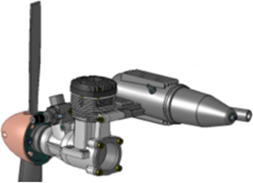
\includegraphics[width=.45\textwidth]{fig_00}
}%figues de la page de garde
\def\xxpied{%
Révisions Statique -- Arcboutement\\% afin de valider leurs performances.\\
Révisions 2 -- \xxactivite%
}

\iflivret
\pagestyle{empty}


%%%%%%%% PAGE DE GARDE COURS
\ifcours
% ==== BANDEAU DES TITRES ==== 
\begin{tikzpicture}[remember picture,overlay]
\node at (current page.north west)
{\begin{tikzpicture}[remember picture,overlay]
\node[anchor=north west,inner sep=0pt] at (0,0) {\includegraphics[width=\paperwidth]{\thechapterimage}};
\draw[anchor=west] (-2cm,-8cm) node [line width=2pt,rounded corners=15pt,draw=ocre,fill=white,fill opacity=0.6,inner sep=40pt]{\strut\makebox[22cm]{}};
\draw[anchor=west] (1cm,-8cm) node {\huge\sffamily\bfseries\color{black} %
\begin{minipage}{1cm}
\rotatebox{90}{\LARGE\sffamily\textsc{\color{ocre}\textbf{\xxnumpartie}}}
\end{minipage} \hfill
\begin{minipage}[c]{14cm}
\begin{titrepartie}
\begin{flushright}
\renewcommand{\baselinestretch}{1.1} 
\Large\sffamily\textsc{\textbf{\xxpartie}}
\renewcommand{\baselinestretch}{1} 
\end{flushright}
\end{titrepartie}
\end{minipage} \hfill
\begin{minipage}[c]{3.5cm}
{\large\sffamily\textsc{\textbf{\color{ocre} \discipline}}}
\end{minipage} 
 };
\end{tikzpicture}};
\end{tikzpicture}
% ==== FIN BANDEAU DES TITRES ==== 


% ==== ONGLET 
\begin{tikzpicture}[overlay]
\node[shape=rectangle, 
      rounded corners = .25 cm,
	  draw= ocre,
	  line width=2pt, 
	  fill = ocre!10,
	  minimum width  = 2.5cm,
	  minimum height = 3cm,] at (18.3cm,0) {};
\node at (17.7cm,0) {\rotatebox{90}{\textbf{\Large\color{ocre}{\classe}}}};
%{};
\end{tikzpicture}
% ==== FIN ONGLET 


\vspace{3.5cm}

\begin{tikzpicture}[remember picture,overlay]
\draw[anchor=west] (-2cm,-6cm) node {\huge\sffamily\bfseries\color{black} %
\begin{minipage}{2cm}
\begin{center}
\LARGE\sffamily\textsc{\color{ocre}\textbf{\xxactivite}}
\end{center}
\end{minipage} \hfill
\begin{minipage}[c]{15cm}
\begin{titrechapitre}
\renewcommand{\baselinestretch}{1.1} 
\Large\sffamily\textsc{\textbf{\xxnumchapitre}}

\Large\sffamily\textsc{\textbf{\xxchapitre}}
\vspace{.5cm}

\renewcommand{\baselinestretch}{1} 
\normalsize\normalfont
\xxcompetences
\end{titrechapitre}
\end{minipage}  };
\end{tikzpicture}
\vfill

\begin{flushright}
\begin{minipage}[c]{.3\linewidth}
\begin{center}
\xxfigures
\end{center}
\end{minipage}\hfill
\begin{minipage}[c]{.6\linewidth}
\startcontents
%\printcontents{}{1}{}
\printcontents{}{1}{}
\end{minipage}
\end{flushright}

\begin{tikzpicture}[remember picture,overlay]
\draw[anchor=west] (4.5cm,-.7cm) node {
\begin{minipage}[c]{.2\linewidth}
\begin{flushright}

\includegraphics[width=2cm]{logoCC}
\end{flushright}
\end{minipage}
\begin{minipage}[c]{.2\linewidth}
\textsl{\xxauteur} \\
\textsl{\classe}
\end{minipage}
 };
\end{tikzpicture}

\newpage
\pagestyle{fancy}

%\newpage
%\pagestyle{fancy}

\else
\fi
%% FIN PAGE DE GARDE DES COURS

%%%%%%%% PAGE DE GARDE TD
\iftd
%\begin{tikzpicture}[remember picture,overlay]
%\node at (current page.north west)
%{\begin{tikzpicture}[remember picture,overlay]
%\draw[anchor=west] (-2cm,-3.25cm) node [line width=2pt,rounded corners=15pt,draw=ocre,fill=white,fill opacity=0.6,inner sep=40pt]{\strut\makebox[22cm]{}};
%\draw[anchor=west] (1cm,-3.25cm) node {\huge\sffamily\bfseries\color{black} %
%\begin{minipage}{1cm}
%\rotatebox{90}{\LARGE\sffamily\textsc{\color{ocre}\textbf{\xxnumpartie}}}
%\end{minipage} \hfill
%\begin{minipage}[c]{13.5cm}
%\begin{titrepartie}
%\begin{flushright}
%\renewcommand{\baselinestretch}{1.1} 
%\Large\sffamily\textsc{\textbf{\xxpartie}}
%\renewcommand{\baselinestretch}{1} 
%\end{flushright}
%\end{titrepartie}
%\end{minipage} \hfill
%\begin{minipage}[c]{3.5cm}
%{\large\sffamily\textsc{\textbf{\color{ocre} \discipline}}}
%\end{minipage} 
% };
%\end{tikzpicture}};
%\end{tikzpicture}

%%%%%%%%%% PAGE DE GARDE TD %%%%%%%%%%%%%%%
%\begin{tikzpicture}[overlay]
%\node[shape=rectangle, 
%      rounded corners = .25 cm,
%	  draw= ocre,
%	  line width=2pt, 
%	  fill = ocre!10,
%	  minimum width  = 2.5cm,
%	  minimum height = 2.5cm,] at (18.5cm,0) {};
%\node at (17.7cm,0) {\rotatebox{90}{\textbf{\Large\color{ocre}{\classe}}}};
%%{};
%\end{tikzpicture}

% PARTIE ET CHAPITRE
%\begin{tikzpicture}[remember picture,overlay]
%\draw[anchor=west] (-1cm,-2.1cm) node {\large\sffamily\bfseries\color{black} %
%\begin{minipage}[c]{15cm}
%\begin{flushleft}
%\xxnumchapitre \\
%\xxchapitre
%\end{flushleft}
%\end{minipage}  };
%\end{tikzpicture}

% BANDEAU EXO
\iflivret % SI LIVRET
\begin{tikzpicture}[remember picture,overlay]
\draw[anchor=west] (-2cm,-3.3cm) node {\huge\sffamily\bfseries\color{black} %
\begin{minipage}{5cm}
\begin{center}
\LARGE\sffamily\color{ocre}\textbf{\textsc{\xxactivite}}

\begin{center}
\xxfigures
\end{center}

\end{center}
\end{minipage} \hfill
\begin{minipage}[c]{12cm}
\begin{titrechapitre}
\renewcommand{\baselinestretch}{1.1} 
\large\sffamily\textbf{\textsc{\xxtitreexo}}

\small\sffamily{\textbf{\textit{\color{black!70}\xxsourceexo}}}
\vspace{.5cm}

\renewcommand{\baselinestretch}{1} 
\normalsize\normalfont
\xxcompetences
\end{titrechapitre}
\end{minipage}};
\end{tikzpicture}
\else % ELSE NOT LIVRET
\begin{tikzpicture}[remember picture,overlay]
\draw[anchor=west] (-2cm,-4.5cm) node {\huge\sffamily\bfseries\color{black} %
\begin{minipage}{5cm}
\begin{center}
\LARGE\sffamily\color{ocre}\textbf{\textsc{\xxactivite}}

\begin{center}
\xxfigures
\end{center}

\end{center}
\end{minipage} \hfill
\begin{minipage}[c]{12cm}
\begin{titrechapitre}
\renewcommand{\baselinestretch}{1.1} 
\large\sffamily\textbf{\textsc{\xxtitreexo}}

\small\sffamily{\textbf{\textit{\color{black!70}\xxsourceexo}}}
\vspace{.5cm}

\renewcommand{\baselinestretch}{1} 
\normalsize\normalfont
\xxcompetences
\end{titrechapitre}
\end{minipage}};
\end{tikzpicture}

\fi

\else   % FIN IF TD
\fi


%%%%%%%% PAGE DE GARDE FICHE
\iffiche
\begin{tikzpicture}[remember picture,overlay]
\node at (current page.north west)
{\begin{tikzpicture}[remember picture,overlay]
\draw[anchor=west] (-2cm,-2.25cm) node [line width=2pt,rounded corners=15pt,draw=ocre,fill=white,fill opacity=0.6,inner sep=40pt]{\strut\makebox[22cm]{}};
\draw[anchor=west] (1cm,-2.25cm) node {\huge\sffamily\bfseries\color{black} %
\begin{minipage}{1cm}
\rotatebox{90}{\LARGE\sffamily\textsc{\color{ocre}\textbf{\xxnumpartie}}}
\end{minipage} \hfill
\begin{minipage}[c]{14cm}
\begin{titrepartie}
\begin{flushright}
\renewcommand{\baselinestretch}{1.1} 
\large\sffamily\textsc{\textbf{\xxpartie} \\} 

\vspace{.2cm}

\normalsize\sffamily\textsc{\textbf{\xxnumchapitre -- \xxchapitre}}
\renewcommand{\baselinestretch}{1} 
\end{flushright}
\end{titrepartie}
\end{minipage} \hfill
\begin{minipage}[c]{3.5cm}
{\large\sffamily\textsc{\textbf{\color{ocre} \discipline}}}
\end{minipage} 
 };
\end{tikzpicture}};
\end{tikzpicture}

\iflivret
\begin{tikzpicture}[overlay]
\node[shape=rectangle, 
      rounded corners = .25 cm,
	  draw= ocre,
	  line width=2pt, 
	  fill = ocre!10,
	  minimum width  = 2.5cm,
	  minimum height = 2.5cm,] at (18.5cm,.5cm) {};
\node at (17.9cm,.5cm) {\rotatebox{90}{\textsf{\textbf{\large\color{ocre}{\classe}}}}};
%{};
\end{tikzpicture}
\else
\begin{tikzpicture}[overlay]
\node[shape=rectangle, 
      rounded corners = .25 cm,
	  draw= ocre,
	  line width=2pt, 
	  fill = ocre!10,
	  minimum width  = 2.5cm,
%	  minimum height = 2.5cm,] at (18.5cm,1.1cm) {};
	  minimum height = 2.5cm,] at (18.6cm,0.5cm) {};
\node at (18cm,0.5cm) {\rotatebox{90}{\textsf{\textbf{\large\color{ocre}{\classe}}}}};
%{};
\end{tikzpicture}

\fi

\else
\fi



\else
\pagestyle{empty}


%%%%%%%% PAGE DE GARDE COURS
\ifcours
% ==== BANDEAU DES TITRES ==== 
\begin{tikzpicture}[remember picture,overlay]
\node at (current page.north west)
{\begin{tikzpicture}[remember picture,overlay]
\node[anchor=north west,inner sep=0pt] at (0,0) {\includegraphics[width=\paperwidth]{\thechapterimage}};
\draw[anchor=west] (-2cm,-8cm) node [line width=2pt,rounded corners=15pt,draw=ocre,fill=white,fill opacity=0.6,inner sep=40pt]{\strut\makebox[22cm]{}};
\draw[anchor=west] (1cm,-8cm) node {\huge\sffamily\bfseries\color{black} %
\begin{minipage}{1cm}
\rotatebox{90}{\LARGE\sffamily\textsc{\color{ocre}\textbf{\xxnumpartie}}}
\end{minipage} \hfill
\begin{minipage}[c]{14cm}
\begin{titrepartie}
\begin{flushright}
\renewcommand{\baselinestretch}{1.1} 
\Large\sffamily\textsc{\textbf{\xxpartie}}
\renewcommand{\baselinestretch}{1} 
\end{flushright}
\end{titrepartie}
\end{minipage} \hfill
\begin{minipage}[c]{3.5cm}
{\large\sffamily\textsc{\textbf{\color{ocre} \discipline}}}
\end{minipage} 
 };
\end{tikzpicture}};
\end{tikzpicture}
% ==== FIN BANDEAU DES TITRES ==== 


% ==== ONGLET 
\begin{tikzpicture}[overlay]
\node[shape=rectangle, 
      rounded corners = .25 cm,
	  draw= ocre,
	  line width=2pt, 
	  fill = ocre!10,
	  minimum width  = 2.5cm,
	  minimum height = 3cm,] at (18.3cm,0) {};
\node at (17.7cm,0) {\rotatebox{90}{\textbf{\Large\color{ocre}{\classe}}}};
%{};
\end{tikzpicture}
% ==== FIN ONGLET 


\vspace{3.5cm}

\begin{tikzpicture}[remember picture,overlay]
\draw[anchor=west] (-2cm,-6cm) node {\huge\sffamily\bfseries\color{black} %
\begin{minipage}{2cm}
\begin{center}
\LARGE\sffamily\textsc{\color{ocre}\textbf{\xxactivite}}
\end{center}
\end{minipage} \hfill
\begin{minipage}[c]{15cm}
\begin{titrechapitre}
\renewcommand{\baselinestretch}{1.1} 
\Large\sffamily\textsc{\textbf{\xxnumchapitre}}

\Large\sffamily\textsc{\textbf{\xxchapitre}}
\vspace{.5cm}

\renewcommand{\baselinestretch}{1} 
\normalsize\normalfont
\xxcompetences
\end{titrechapitre}
\end{minipage}  };
\end{tikzpicture}
\vfill

\begin{flushright}
\begin{minipage}[c]{.3\linewidth}
\begin{center}
\xxfigures
\end{center}
\end{minipage}\hfill
\begin{minipage}[c]{.6\linewidth}
\startcontents
%\printcontents{}{1}{}
\printcontents{}{1}{}
\end{minipage}
\end{flushright}

\begin{tikzpicture}[remember picture,overlay]
\draw[anchor=west] (4.5cm,-.7cm) node {
\begin{minipage}[c]{.2\linewidth}
\begin{flushright}

\includegraphics[width=2cm]{logoCC}
\end{flushright}
\end{minipage}
\begin{minipage}[c]{.2\linewidth}
\textsl{\xxauteur} \\
\textsl{\classe}
\end{minipage}
 };
\end{tikzpicture}

\newpage
\pagestyle{fancy}

%\newpage
%\pagestyle{fancy}

\else
\fi
%% FIN PAGE DE GARDE DES COURS

%%%%%%%% PAGE DE GARDE TD
\iftd
%\begin{tikzpicture}[remember picture,overlay]
%\node at (current page.north west)
%{\begin{tikzpicture}[remember picture,overlay]
%\draw[anchor=west] (-2cm,-3.25cm) node [line width=2pt,rounded corners=15pt,draw=ocre,fill=white,fill opacity=0.6,inner sep=40pt]{\strut\makebox[22cm]{}};
%\draw[anchor=west] (1cm,-3.25cm) node {\huge\sffamily\bfseries\color{black} %
%\begin{minipage}{1cm}
%\rotatebox{90}{\LARGE\sffamily\textsc{\color{ocre}\textbf{\xxnumpartie}}}
%\end{minipage} \hfill
%\begin{minipage}[c]{13.5cm}
%\begin{titrepartie}
%\begin{flushright}
%\renewcommand{\baselinestretch}{1.1} 
%\Large\sffamily\textsc{\textbf{\xxpartie}}
%\renewcommand{\baselinestretch}{1} 
%\end{flushright}
%\end{titrepartie}
%\end{minipage} \hfill
%\begin{minipage}[c]{3.5cm}
%{\large\sffamily\textsc{\textbf{\color{ocre} \discipline}}}
%\end{minipage} 
% };
%\end{tikzpicture}};
%\end{tikzpicture}

%%%%%%%%%% PAGE DE GARDE TD %%%%%%%%%%%%%%%
%\begin{tikzpicture}[overlay]
%\node[shape=rectangle, 
%      rounded corners = .25 cm,
%	  draw= ocre,
%	  line width=2pt, 
%	  fill = ocre!10,
%	  minimum width  = 2.5cm,
%	  minimum height = 2.5cm,] at (18.5cm,0) {};
%\node at (17.7cm,0) {\rotatebox{90}{\textbf{\Large\color{ocre}{\classe}}}};
%%{};
%\end{tikzpicture}

% PARTIE ET CHAPITRE
%\begin{tikzpicture}[remember picture,overlay]
%\draw[anchor=west] (-1cm,-2.1cm) node {\large\sffamily\bfseries\color{black} %
%\begin{minipage}[c]{15cm}
%\begin{flushleft}
%\xxnumchapitre \\
%\xxchapitre
%\end{flushleft}
%\end{minipage}  };
%\end{tikzpicture}

% BANDEAU EXO
\iflivret % SI LIVRET
\begin{tikzpicture}[remember picture,overlay]
\draw[anchor=west] (-2cm,-3.3cm) node {\huge\sffamily\bfseries\color{black} %
\begin{minipage}{5cm}
\begin{center}
\LARGE\sffamily\color{ocre}\textbf{\textsc{\xxactivite}}

\begin{center}
\xxfigures
\end{center}

\end{center}
\end{minipage} \hfill
\begin{minipage}[c]{12cm}
\begin{titrechapitre}
\renewcommand{\baselinestretch}{1.1} 
\large\sffamily\textbf{\textsc{\xxtitreexo}}

\small\sffamily{\textbf{\textit{\color{black!70}\xxsourceexo}}}
\vspace{.5cm}

\renewcommand{\baselinestretch}{1} 
\normalsize\normalfont
\xxcompetences
\end{titrechapitre}
\end{minipage}};
\end{tikzpicture}
\else % ELSE NOT LIVRET
\begin{tikzpicture}[remember picture,overlay]
\draw[anchor=west] (-2cm,-4.5cm) node {\huge\sffamily\bfseries\color{black} %
\begin{minipage}{5cm}
\begin{center}
\LARGE\sffamily\color{ocre}\textbf{\textsc{\xxactivite}}

\begin{center}
\xxfigures
\end{center}

\end{center}
\end{minipage} \hfill
\begin{minipage}[c]{12cm}
\begin{titrechapitre}
\renewcommand{\baselinestretch}{1.1} 
\large\sffamily\textbf{\textsc{\xxtitreexo}}

\small\sffamily{\textbf{\textit{\color{black!70}\xxsourceexo}}}
\vspace{.5cm}

\renewcommand{\baselinestretch}{1} 
\normalsize\normalfont
\xxcompetences
\end{titrechapitre}
\end{minipage}};
\end{tikzpicture}

\fi

\else   % FIN IF TD
\fi


%%%%%%%% PAGE DE GARDE FICHE
\iffiche
\begin{tikzpicture}[remember picture,overlay]
\node at (current page.north west)
{\begin{tikzpicture}[remember picture,overlay]
\draw[anchor=west] (-2cm,-2.25cm) node [line width=2pt,rounded corners=15pt,draw=ocre,fill=white,fill opacity=0.6,inner sep=40pt]{\strut\makebox[22cm]{}};
\draw[anchor=west] (1cm,-2.25cm) node {\huge\sffamily\bfseries\color{black} %
\begin{minipage}{1cm}
\rotatebox{90}{\LARGE\sffamily\textsc{\color{ocre}\textbf{\xxnumpartie}}}
\end{minipage} \hfill
\begin{minipage}[c]{14cm}
\begin{titrepartie}
\begin{flushright}
\renewcommand{\baselinestretch}{1.1} 
\large\sffamily\textsc{\textbf{\xxpartie} \\} 

\vspace{.2cm}

\normalsize\sffamily\textsc{\textbf{\xxnumchapitre -- \xxchapitre}}
\renewcommand{\baselinestretch}{1} 
\end{flushright}
\end{titrepartie}
\end{minipage} \hfill
\begin{minipage}[c]{3.5cm}
{\large\sffamily\textsc{\textbf{\color{ocre} \discipline}}}
\end{minipage} 
 };
\end{tikzpicture}};
\end{tikzpicture}

\iflivret
\begin{tikzpicture}[overlay]
\node[shape=rectangle, 
      rounded corners = .25 cm,
	  draw= ocre,
	  line width=2pt, 
	  fill = ocre!10,
	  minimum width  = 2.5cm,
	  minimum height = 2.5cm,] at (18.5cm,.5cm) {};
\node at (17.9cm,.5cm) {\rotatebox{90}{\textsf{\textbf{\large\color{ocre}{\classe}}}}};
%{};
\end{tikzpicture}
\else
\begin{tikzpicture}[overlay]
\node[shape=rectangle, 
      rounded corners = .25 cm,
	  draw= ocre,
	  line width=2pt, 
	  fill = ocre!10,
	  minimum width  = 2.5cm,
%	  minimum height = 2.5cm,] at (18.5cm,1.1cm) {};
	  minimum height = 2.5cm,] at (18.6cm,0.5cm) {};
\node at (18cm,0.5cm) {\rotatebox{90}{\textsf{\textbf{\large\color{ocre}{\classe}}}}};
%{};
\end{tikzpicture}

\fi

\else
\fi



\fi
\setlength{\columnseprule}{.1pt}

\pagestyle{fancy}
\thispagestyle{plain}

\vspace{5cm}

\def\columnseprulecolor{\color{ocre}}
\setlength{\columnseprule}{0.4pt} 

\setcounter{exo}{0}

%%%%%%%%%%%%%%%%%%%%%%%%%%%%%%%%%%%%%%%%%%%%%%%%%%

\ifprof
\else
\begin{multicols}{2}
\fi

\subsection*{Mise en situation}
\ifprof
\else
Le système EOS permet l’acquisition simultanée de radiographies de face et de profil du corps entier (ou d’une zone anatomique localisée) avec une réduction de la dose de rayons X de l’ordre de 90\,\% par rapport à un système radiographique conventionnel ou un scanner.


\begin{center}
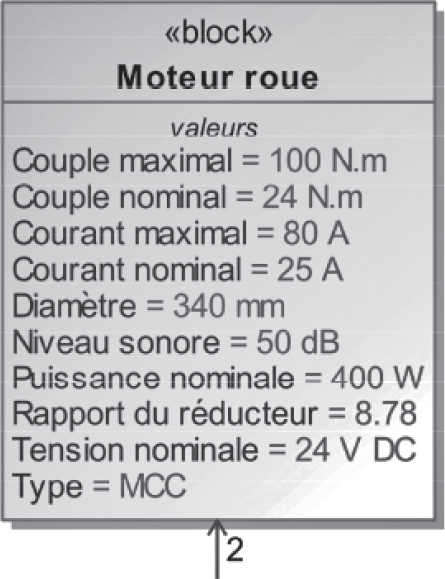
\includegraphics[width=.7\linewidth]{fig_02}
%\textit{}
\end{center}

Le mécanisme interne, constitué d’un bras mobile, guidé par rapport au bâti par trois colonnes
verticales. Le bras supporte deux chaînes d’acquisition, chacune d’entre elles étant composée d’un tube à rayons X et d’un détecteur.

\begin{center}
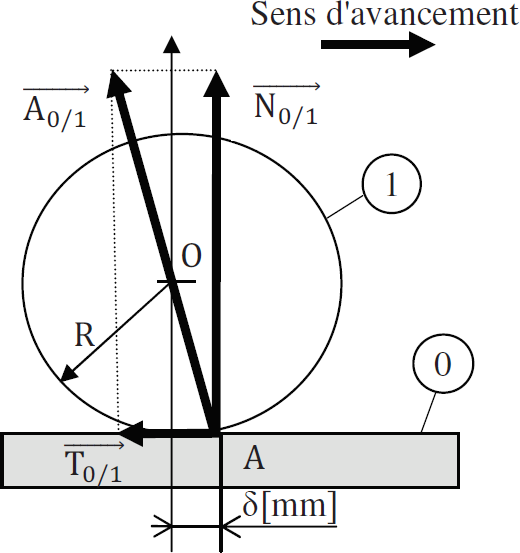
\includegraphics[width=.7\linewidth]{fig_03}
%\textit{}
\end{center}


La figure suivante représente le bras mobile en vue de dessus, ce qui permet de voir les passages des colonnes et
des vis. Le modèle cinématique permettant d’appréhender le fonctionnement interne. 


\begin{center}
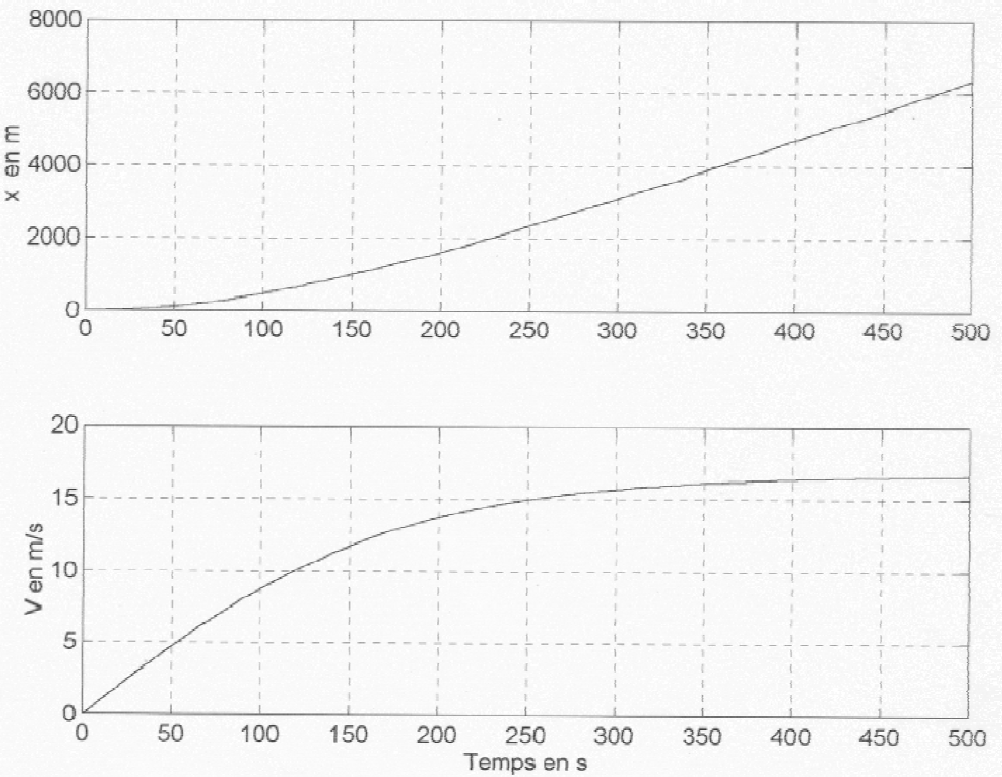
\includegraphics[width=.7\linewidth]{fig_04}
%\textit{}
\end{center}





On s’intéresse plus précisément à une des trois chaînes réalisant la liaison entre le bras mobile 1 et le bâti
0. 
Cette liaison est principalement réalisée par le biais d’une colonne 2, qui est en liaison complète avec 0. Un schéma de principe est représenté sur la figure suivante. La colonne est de diamètre $d$, l’alésage du bras de diamètre
$d + j$ et  de longueur $\ell$. On suppose que le jeu $j$, bien que négligeable devant d ($j  \ll d$ ), permet un léger
basculement du bras par rapport à la colonne, ce qui conduit à considérer cet assemblage comme l’association en parallèle de deux liaisons sphère-plan, en $I$ et $J$. Le contact est modélisé en utilisant la modèle de Coulomb et on note $f$  le coefficient  de frottement. Le bras 1 est soumis à une action mécanique motrice (issue de la
liaison hélicoïdale) modélisée par un glisseur en $B$ noté $F = -F_z$ ($F > 0$) dont l’axe central est distant de $e$
de l’axe de la liaison. On se propose  d’étudier le risque d’arcboutement  de cette liaison, supposée plane, en négligeant les actions de la pesanteur.

\fi

\begin{obj}
Déterminer les conditions de non arcboutement du guidage du système EOS. 
\end{obj}


\ifprof
\else
\begin{center}
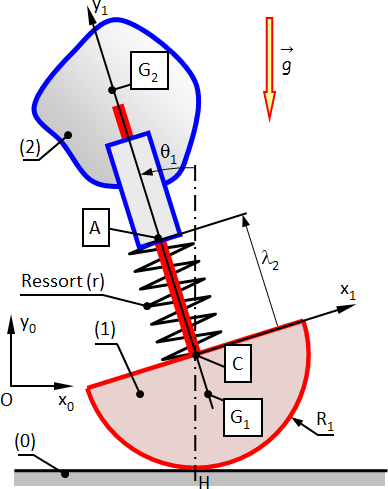
\includegraphics[width=\linewidth]{fig_01}
%\textit{}
\end{center}

\fi

\subsection*{Travail à réaliser}
\subparagraph{}\textit{En introduisant $F_I = Y_ I \vect{y} + Z_ I \vect{z}$ et $F_J = Y_ J \vect{y} + Z_ J \vect{z}$, les glisseurs en $I$ et $J$ qui résultent des actions mécaniques exercées par la colonne 2 sur le bras 1, écrire les trois équations scalaires traduisant l’équilibre du bras.}
\ifprof
\begin{corrige}~\\

En appliquant le PFS en $B$, on a : 

$\left\{
\begin{array}{l}
Y_I + Y_J = 0 \\
Z_I + Z_J -F = 0 \\ 
-Y_J \dfrac{\ell}{2}-Z_J \left(e+\dfrac{d}{2}\right) 
+Y_I \dfrac{\ell}{2}-Z_I \left(e-\dfrac{d}{2}\right) = 0
\end{array}
\right.$
%
%$
%\Leftrightarrow
%\left\{
%\begin{array}{l}
%Y_I + Y_J = 0 \\
%Z_I + Z_J -F = 0 \\ 
%d Z_J = -\left(e-\dfrac{d}{2}\right)F -\ell Y_J 
%\end{array}
%\right.$
\end{corrige}


%\begin{corrige}~\\
%
%En appliquant le PFS en $I$, on a : 
%
%$\left\{
%\begin{array}{l}
%Y_I + Y_J = 0 \\
%Z_I + Z_J -F = 0 \\ 
%-\left(e-\dfrac{d}{2}\right)F -\ell Y_J -d Z_J = 0
%\end{array}
%\right.$
%
%$
%\Leftrightarrow
%\left\{
%\begin{array}{l}
%Y_I + Y_J = 0 \\
%Z_I + Z_J -F = 0 \\ 
%d Z_J = -\left(e-\dfrac{d}{2}\right)F -\ell Y_J 
%\end{array}
%\right.$
%\end{corrige}

\else
\fi


\subparagraph{}\textit{En supposant que $F > 0$, comme précisé ci-dessus, donner  les signes des composantes  $Y_I$, $Z_I$, $Y_J$ et $Z_J$ puis écrire,  en utilisant  le modèle  de Coulomb, les inéquations  qui lient ces composantes.}
\ifprof
\begin{corrige} ~\\
On a de plus : 
$
\left\{
\begin{array}{l}
Y_I \geq 0 \text{ et } Z_I \geq 0 \\
Y_J \leq 0 \text{ et } Z_J \geq 0 \\
|Z_I|\leq f|Y_I| \text{ et }  |Z_J|\leq f|Y_J| \\
\end{array}
\right.$
$ \Rightarrow 
\left\{
\begin{array}{l}
Y_I \geq 0 \text{ et } Z_I \geq 0 \\
Y_J \leq 0 \text{ et } Z_J \geq 0 \\
Z_I\leq fY_I \text{ et }  Z_J\leq -fY_J \\
\end{array}
\right.$


\end{corrige}
\else
\fi

\subparagraph{}\textit{En supposant qu’on est à  la limite du glissement au niveau d’un des contacts, donner la condition nécessaire entre $\ell$, $f$ et $e$ pour qu’il n’y ait pas d’arcboutement dans la liaison.}

\ifprof
\begin{corrige}~\\

\textbf{On considère qu'on est à la limite du glissement au point $I$.}
  En conséquences, 

$
\left\{
\begin{array}{l}
Z_I =  fY_I  \\
Y_I + Y_J = 0 \\
Z_I + Z_J -F = 0 \\ 
-Y_J \dfrac{\ell}{2}-Z_J \left(e+\dfrac{d}{2}\right) 
+Y_I \dfrac{\ell}{2}-Z_I \left(e-\dfrac{d}{2}\right) = 0
\end{array}
\right.$
$
\Leftrightarrow
\left\{
\begin{array}{l}
Z_I =  fY_I  \\
Y_J = -Y_I \\
Z_J=F-Z_I =F-fY_I  \\ 
Y_I \dfrac{\ell}{2}-\left( F-fY_I\right) \left(e+\dfrac{d}{2}\right) 
+Y_I \dfrac{\ell}{2}-fY_I \left(e-\dfrac{d}{2}\right) = 0
\end{array}
\right.$

$Y_I \dfrac{\ell}{2}-\left( F-fY_I\right) \left(e+\dfrac{d}{2}\right) 
+Y_I \dfrac{\ell}{2}-fY_I \left(e-\dfrac{d}{2}\right) = 0$

$\Leftrightarrow Y_I\left(  \dfrac{\ell}{2}+ f \left(e+\dfrac{d}{2}\right) 
+\dfrac{\ell}{2}-f \left(e-\dfrac{d}{2}\right)\right) - F\left(e+\dfrac{d}{2}\right) = 0$

$\Leftrightarrow Y_I\left(  \ell+fd \right) - F\left(e+\dfrac{d}{2}\right) = 0$
 
 et $\Leftrightarrow F = Y_I \dfrac{\ell+fd }{e+\dfrac{d}{2}}= Y_I \dfrac{2\ell+2fd }{2e+d}$

De plus, au point $J$, on a nécessairement : 
$Z_J\leq -fY_J $. En conséquences, 

$F-fY_I \leq fY_I $

$\Leftrightarrow F-fY_I \leq fY_I $
$\Leftrightarrow F \leq 2fY_I $
$\Leftrightarrow F \leq 2fY_I $
$\Leftrightarrow  Y_I \dfrac{2\ell+2fd }{2e+d}\leq 2fY_I $
$\Leftrightarrow  \dfrac{2\ell+2fd }{2e+d}\leq 2f$
$\Leftrightarrow  2\ell+2fd \leq 4f e+2fd $
$\Leftrightarrow  \ell \leq 2f e $
$\Leftrightarrow  \dfrac{\ell}{2e} \leq f $
\end{corrige}

\begin{corrige}~\\

\textbf{On considère qu'on est à la limite du glissement au point $J$.}
  En conséquences, 

$
\left\{
\begin{array}{l}
Z_J =  -fY_J \\
Y_I + Y_J = 0 \\
Z_I + Z_J -F = 0 \\ 
-Y_J \dfrac{\ell}{2}-Z_J \left(e+\dfrac{d}{2}\right) 
+Y_I \dfrac{\ell}{2}-Z_I \left(e-\dfrac{d}{2}\right) = 0
\end{array}
\right.$

$
\Leftrightarrow 
\left\{
\begin{array}{l}
Z_J =  -fY_J \\
Y_I =- Y_J  \\
Z_I = -Z_J +F  = fY_J +F \\ 
-Y_J \dfrac{\ell}{2}+fY_J \left(e+\dfrac{d}{2}\right) 
-Y_J \dfrac{\ell}{2}-\left(  fY_J +F\right) \left(e-\dfrac{d}{2}\right) = 0
\end{array}
\right.$

Et donc $Y_J\left(- {\ell}+f \left(e+\dfrac{d}{2}\right) 
- f  \left(e-\dfrac{d}{2}\right)\right) 
-F \left(e-\dfrac{d}{2}\right)= 0$
$\Leftrightarrow Y_J\left(- {\ell}+f d\right) -F \left(e-\dfrac{d}{2}\right)= 0$
$\Leftrightarrow Y_J\left(- {\ell}+f d\right) =F \left(e-\dfrac{d}{2}\right)$
$\Leftrightarrow F = Y_J\dfrac{- {\ell}+f d}{e-\dfrac{d}{2}}$

Par ailleurs, on a : 
$Z_I\leq fY_I$ 
$\Leftrightarrow   fY_J +F \leq -f  Y_J$

$\Leftrightarrow   2fY_J +F \leq 0$
$\Leftrightarrow   2fY_J +Y_J\dfrac{- {\ell}+f d}{e-\dfrac{d}{2}} \leq 0$
$\Leftrightarrow   2f +\dfrac{- {\ell}+f d}{e-\dfrac{d}{2}} \geq 0$ ($Y_J<0$)
$\Leftrightarrow   \dfrac{2fe-fd- {\ell}+f d}{e-\dfrac{d}{2}} \geq 0$ 
$\Leftrightarrow   \dfrac{2fe- {\ell}}{e-\dfrac{d}{2}} \geq 0$ . 


???

\begin{itemize}
\item Si $e-\dfrac{d}{2}>0$ : ${2fe- {\ell}} \geq 0$ et  $f \geq \dfrac{{\ell}}{2e}$.
\item Si $e-\dfrac{d}{2}<0$ : ${2fe- {\ell}} \leq 0$ et  $f \leq \dfrac{{\ell}}{2e}$.
\end{itemize}
\end{corrige}


%\begin{corrige}~\\
%
%On considère qu'on est à la limite du glissement au point $I$.  En conséquences, 
%
%$
%\left\{
%\begin{array}{l}
%Z_I =  fY_I  \\
%Y_I + Y_J = 0 \\
%Z_I + Z_J -F = 0 \\ 
%-\left(e-\dfrac{d}{2}\right)F -\ell Y_J -d Z_J = 0
%\end{array}
%\right.$
%
%$\Rightarrow
%\left\{
%\begin{array}{l}
%Z_I =  fY_I  \\
%Y_I =- Y_J \\
%Z_I + Z_J -F = 0 \Leftrightarrow  - f Y_J + Z_J -F = 0\Leftrightarrow  f Y_J =  Z_J -F  \\ 
%-\left(e-\dfrac{d}{2}\right)F -\ell \dfrac{Z_J -F}{f}  -d Z_J = 0
%\end{array}
%\right.$
%
%On a donc
% $-\left(e-\dfrac{d}{2}\right)F - \dfrac{\ell Z_J }{f}  + \dfrac{ \ell F}{f}   -d Z_J = 0$
% 
% $\Leftrightarrow -\left(e-\dfrac{d}{2} + \dfrac{ \ell}{f} \right)F -\left( \dfrac{\ell }{f}+d \right)Z_J = 0$
% 
% $\Leftrightarrow -\left(e-\dfrac{d}{2} + \dfrac{ \ell}{f} \right)F =\left( \dfrac{\ell }{f}+d \right)Z_J $
% 
% $ \Leftrightarrow Z_J = \dfrac{-2fe+fd - 2\ell}{2\ell +2fd} F  $
% 
% 
% De plus, on a : 
%$ Z_J\leq -fY_J$ 
%$\Leftrightarrow \dfrac{-2fe+fd - 2\ell}{2\ell +2fd} F  \leq   F-Z_J $ 
%$\Leftrightarrow \dfrac{-2fe+fd - 2\ell}{2\ell +2fd} F  \leq   F- \dfrac{-2fe+fd - 2\ell}{2\ell +2fd} F  $ 
%
%$\Leftrightarrow \dfrac{-2fe+fd - 2\ell}{2\ell +2fd}   \leq   \dfrac{2\ell +2fd+2fe-fd + 2\ell}{2\ell +2fd}   $ 
%
%$\Leftrightarrow -2fe+fd - 2\ell   \leq   2\ell +2fd+2fe-fd + 2\ell $ 
%
%$\Leftrightarrow 0    \leq   6\ell +4fe $ 
%$\Leftrightarrow 0    \leq   3\ell +2fe $ 
%
%
%\end{corrige}

%\begin{corrige}~\\
%
%On considère qu'on est à la limite du glissement au point $J$.  En conséquences, 
%
%$
%\left\{
%\begin{array}{l}
%Z_J =  fY_J  \\
%Y_I + Y_J = 0 \Leftrightarrow  Y_I =- Y_J \\
%Z_I + Z_J -F = 0 \Leftrightarrow   Z_I = - Z_J +F = - fY_J +F\\ 
%-\left(e-\dfrac{d}{2}\right)F -\ell Y_J -d Z_J = 0
%\end{array}
%\right.$
%$ \Leftrightarrow
%\left\{
%\begin{array}{l}
%Z_J =  fY_J  \\
%Y_I + Y_J = 0 \Leftrightarrow  Y_I =- Y_J \\
%Z_I + Z_J -F = 0 \Leftrightarrow   Z_I = - Z_J +F = - fY_J +F\\ 
%-\left(e-\dfrac{d}{2}\right)F -\ell Y_J -d fY_J  = 0
%\end{array}
%\right.$
%
%$ \Leftrightarrow
%\left\{
%\begin{array}{l}
%Z_J =  fY_J  \\
%Y_I + Y_J = 0 \Leftrightarrow  Y_I =- Y_J \\
%Z_I + Z_J -F = 0 \Leftrightarrow   Z_I = - Z_J +F = - fY_J +F\\ 
%\left(e-\dfrac{d}{2}\right)F +\left(\ell  +d f\right)Y_J  = 0
%\end{array}
%\right.$
%$ \Leftrightarrow
%\left\{
%\begin{array}{l}
%Z_J =  fY_J  \\
%Y_I =- Y_J = \dfrac{e-\dfrac{d}{2}}{\ell  +d f}F\\
%Z_I = - fY_J +F=- f \dfrac{\dfrac{d}{2}-e}{\ell  +d f}F +F\\ 
%Y_J  = \dfrac{\dfrac{d}{2}-e}{\ell  +d f}F
%\end{array}
%\right.$
%
%
%$ \Leftrightarrow
%\left\{
%\begin{array}{l}
%Z_J =  fY_J  \\
%Y_I = \dfrac{e-\dfrac{d}{2}}{\ell  +d f}F\\
%Z_I =  \dfrac{fe+\dfrac{fd}{2}+\ell  }{\ell  +d f}F \\ 
%Y_J  = \dfrac{\dfrac{d}{2}-e}{\ell  +d f}F
%\end{array}
%\right.$
%
%De plus,  $Z_I\leq fY_I$.
%
%On a donc,  $\dfrac{fe+\dfrac{fd}{2}+\ell  }{\ell  +d f}F\leq f\dfrac{e-\dfrac{d}{2}}{\ell  +d f}F$
%
%$\Leftrightarrow fe+\dfrac{fd}{2}+\ell  \leq fe-\dfrac{fd}{2}$
%
%$\Leftrightarrow {fd}+\ell  \leq 0$
%
%$\Leftrightarrow {fd}+\ell  \leq 0$
%
%\end{corrige}
\else
\fi


\subsection*{Conclusion vis-à-vis de l'objectif}
\subparagraph{}\textit{Vérifier que la condition de non arcboutement est satisfaite sur le système EOS pour lequel les grandeurs caractéristiques fournies ci-dessous ?}
\ifprof
\begin{corrige}
Pour ne pas arcbouter, il faut donc vérifier la relation $\dfrac{\ell}{2e} > f $ : $\dfrac{20}{2\times 20} > f $ et donc $0,5>0,2$.  La condition de glissement est donc vérifiée. 
\end{corrige}
\else
\fi



\ifprof
\else

\footnotesize
\noindent\begin{center}
\begin{tabular}{|p{2.6cm}|c|c|p{1.5cm}|}
\hline
Grandeur & Notation & Unités & Valeur numérique \\ \hline
Diamètre des colonnes  de guidage & d & cm & 10 \\ \hline
Diamètre des vis de guidage & d' & cm & 5 \\ \hline
Hauteur totale des colonnes & H & cm & 200 \\ \hline
Limite de course du bras & h0 & cm & 10 \\ \hline
Longueur de guidage des colonnes & $\ell$  & cm & 20 \\ \hline
Coefficient de frottement colonne/bras & f & -- & 0,2 \\ \hline
Excentration guidage en translation & e & cm & 20 \\ \hline
%Module d’Young des colonnes  de guidage	E	GPa	200 \\ \hline
\end{tabular}
\end{center}

\normalsize
\fi


\ifprof
\else
\begin{center}
\begin{tabular}{|p{.95\linewidth}|}
\hline

\begin{enumerate}
\item $\left\{
\begin{array}{l}
Y_I + Y_J = 0 \\
Z_I + Z_J -F = 0 \\ 
-Y_J \dfrac{\ell}{2}-Z_J \left(e+\dfrac{d}{2}\right) 
+Y_I \dfrac{\ell}{2}-Z_I \left(e-\dfrac{d}{2}\right) = 0
\end{array}
\right.$
\item .
\item $\dfrac{\ell}{2e} \leq f $
\item .
\end{enumerate} \\
\hline
\end{tabular}
\end{center}
\fi

\ifprof
\else
\end{multicols}
\fi
